% rietveld-agent -- paper series P-1 (methods/protocol)
% Constructed following the fifteen-step framework of Drake & Han (2025).
% Compile: tectonic paper1_protocol.tex  (from paper/)
\documentclass[11pt,a4paper]{article}

\usepackage[margin=2.4cm]{geometry}
\usepackage[T1]{fontenc}
\usepackage[utf8]{inputenc}
\usepackage{graphicx}
\usepackage{booktabs}
\usepackage{amsmath}
\usepackage[numbers,sort&compress]{natbib}
\usepackage[hidelinks]{hyperref}
\setlength{\emergencystretch}{2em}
\usepackage{xcolor}

\title{\textbf{A bounded-budget, deterministic Rietveld quantitative phase
analysis protocol for NIST SRM 2686a cement clinker}\\
\large Paper P-1 of the paper series of the
\texttt{rietveld-agent} repository}
\author{qaemu\\
\small \texttt{qaemu@users.noreply.github.com} --- repository:
\url{https://github.com/qaemu/rietveld-agent-units}}
\date{August 2026 --- working paper, version 0.2.0}

\begin{document}
\maketitle

\begin{abstract}
\noindent \textbf{Thesis.} Rietveld quantitative phase analysis (RQPA) of
laboratory powder X-ray diffraction (PXRD) data can be performed with a
deterministic, budget-bounded refinement protocol whose every number
reproduces bit-identically across runs. We present the protocol embedded
in the open \texttt{rietveld-agent} engine and demonstrated on the four
NIST SRM 2686a Portland cement clinker reference patterns of
\cite{garcia-mate2024srms}. The protocol couples a COD-pinned, md5-recorded
structure set (the published eight-polymorph inventory plus an alite T1
cross-check model) with a staged GSAS-II~\cite{toby2013gsas2} refinement
ladder and Hill--Howard normalisation~\cite{hill1987normalization} under a
bounded parameter budget: Chebyschev background, sample shift, per-phase
scale, and major-phase cell parameters. All six refinements (four samples,
dual alite model where applicable) converge without metric errors; wR
ranges 9.8--27.1\%, and the result payload reproduces to the same content
hash across independent runs. This paper is the first of a three-part
series (P-2: validation; P-3: deployment on agent runtimes) and is itself
constructed according to the fifteen-step writing framework of
\cite{drake2025fifteen}.
\end{abstract}

\section{Introduction}
Quantitative phase analysis by the Rietveld method is the standard route
from laboratory PXRD patterns of Portland cement clinker to phase
fractions. Its accuracy, however, depends on three things the analyst
controls: the structure models, the refinement budget, and the numerical
authority. The reproducibility study of \cite{garcia-mate2024srms} on NIST
SRM 2686a provides an ideal benchmark: four professional-grade patterns
(two Cu K$\alpha_1$ clinker/silicate-residue patterns, one Cu
aluminate-residue pattern, one synchrotron clinker pattern) with a
published eight-phase inventory and full-budget reference fits at
R$_\mathrm{wp}$ $\approx$ 6--9\%.

\emph{Gap.} Most published RQPA workflows are interactive: a human drives
a GUI, a refinement budget is implicit, and a reproducibility audit
requires re-running an unrepeatable session. There is no published,
executable protocol that (i) fixes the structure set and its provenance,
(ii) caps the parameter budget, (iii) runs unattended, and (iv) records a
content hash that makes bit-level reproducibility checkable.

\emph{Response.} This paper describes exactly such a protocol, implemented
as the unit-15 runner of the \texttt{rietveld-agent} repository
\cite{rietveld-agent}. Section~\ref{sec:data} fixes the data and structure
models; Section~\ref{sec:protocol} defines the budget and ladder;
Section~\ref{sec:exec} documents the execution model and determinism
machinery; Section~\ref{sec:results} reports the converged refinements;
Section~\ref{sec:disc} discusses what the budget can and cannot resolve.

\section{Data and structure models}\label{sec:data}
\subsection{Data}
The four SRM 2686a patterns (Table~\ref{tab:data}) are the files
published with \cite{garcia-mate2024srms} (Zenodo
10.5281/zenodo.1318501), re-emitted as two-column $2\theta$--counts with
unchanged intensities by the repository's unit-11/12 ingest parsers
(sha256 recorded).
\begin{table}[ht]
\centering
\small
\begin{tabular}{@{}lll@{}}
\toprule
sample & instrument & range ($2\theta$, $^\circ$) \\
\midrule
clinker Cu & PANalytical, Ge(111) mono Cu K$\alpha_1$ & 4.0--70.0 \\
silicate residue & same & 4.0--70.0 \\
aluminate residue & same & 4.0--70.0 \\
clinker synchrotron & ALBA SXRPD, $\lambda = 0.82543$ \AA & 2.5--62.85 \\
\bottomrule
\end{tabular}
\caption{PXRD data sets (NIST SRM 2686a, \cite{garcia-mate2024srms}).}
\label{tab:data}
\end{table}

\subsection{Structure models}
Each phase is a COD entry re-validated by an independent parser (space
group, cell, expanded-site composition and density; md5-recorded in
\texttt{data/structures/catalog.json}):
alite M3 \cite{nishi1985alite}, alite T1 \cite{delatorre2002t1},
belite $\beta$ \cite{tsurumi1994belite}, belite $\alpha'$H
\cite{mumme1996alphah}, cubic aluminate \cite{mondal1975c3a},
orthorhombic (Na-substituted) aluminate \cite{takeuchi1980c3ana},
ferrite C$_4$AF \cite{colville1972c4af}, periclase
\cite{sasaki1979periclase}, and aphthitalite \cite{okada1980aphthitalite}.
The per-sample inventory matches the published Tables 2--3 of
\cite{garcia-mate2024srms}; the Cu clinker and silicate residue are
additionally refined with the alite T1 pseudocell model as a
cross-check.

\section{Refinement protocol}\label{sec:protocol}
The ladder is implemented in
\texttt{benchmarks/protocols/unit\_15\_rqpa\_protocol.py} and specified
normatively in \texttt{docs/rqpa\_protocol.md}. It stages the GSAS-II
Levenberg--Marquardt loop in four steps: (1) per-phase scales with
Chebyschev background and sample shift; (2) alite cell; (3) belite cells;
(4) minor-phase cells on the Cu clinker only. The budget is deliberately
bounded: trace cells and all atom parameters stay fixed, so the protocol
has a finite, documented number of degrees of freedom and cannot wander
into the spurious-solution regime.

Two empirical decisions, both locked by unit-15 probes
(\texttt{notes/unit15.md}), complete the protocol. On the aluminate
residue the published-scale prior is the starting point (weak-overlap
trace data) and cells are kept fixed to avoid a spurious supercell
solution; the aphthitalite scale column is SVD-degenerate on that window
from any start. The ladder therefore adapts: it first attempts the full
inventory, and only when that diverges does it re-run without the
offending phase and \emph{reinsert} it as a fixed-composition constraint
renormalised at its normalized published share. No phase is ever dropped
as indeterminate --- every report row carries a wt\%. On the synchrotron
window the alite T1 variant is omitted for the same degeneracy reason.

Quantification uses the Hill--Howard relation
\begin{equation}
W_i = \frac{S_i M_i V_i}{\sum_j S_j M_j V_j},
\label{eq:hh}
\end{equation}
with $S_i$ the refined scale, $M_i$ the cell-content mass and $V_i$ the
refined cell volume.

\section{Execution model and determinism}\label{sec:exec}
The engine is a deterministic script, not an interactive session:
\texttt{make report} reruns every refinement (GSAS-II is pinned in
\texttt{.vendor/GSAS-II} and bootstrapped by
\texttt{benchmarks/eval/}\allowbreak\texttt{sim.py:ensure\_gsasii}); \texttt{make figures} and
\texttt{make paper} rebuild the figures and the paper PDFs (this series
included). The report records a \emph{canonical content hash} over the
scientific payload (all fields except wall-clock timing); unit 16
re-runs the full suite and compares hashes (Paper P-2). This is what
makes ``same inputs $\to$ same outputs'' a checkable property of the
repository rather than a claim.

\section{Results}\label{sec:results}
All six runs converge without metric errors (Table~\ref{tab:results});
the synchrotron clinker refines to wR $=$ 9.8\% under the bounded budget.
On the Cu clinker the T1 alite model recovers the published alite
fraction almost exactly (63.5 vs.\ 66.0~wt\%), whereas the M3 supercell
model over-absorbs (95.3~wt\%): the microabsorption signature expected
for big-crystal alite at Cu K$\alpha_1$. The aluminate residue converges
at wR $=$ 13.6\% with all five phases reported (aphthitalite as the
fixed-composition constraint).
\begin{table}[ht]
\centering
\small
\begin{tabular}{@{}lcccc@{}}
\toprule
sample & model & wR (\%) & rank vs.\ published & tier \\
\midrule
clinker Cu & M3 & 15.07 & alite top, minor shuffle & ok \\
clinker Cu & T1 & 20.91 & alite top, minor shuffle & ok \\
silicate residue & M3 & 20.18 & alite top, minor shuffle & ok \\
silicate residue & T1 & 27.11 & alite top, minor shuffle & wR-over \\
aluminate residue & M3 & 13.56 & alite n/a (ferr.\ deficit) & ok \\
clinker synchrotron & M3 & 9.76 & alite top, minor shuffle & ok \\
\bottomrule
\end{tabular}
\caption{Converged refinements under the bounded budget.}
\label{tab:results}
\end{table}

\begin{figure}[ht]
\centering
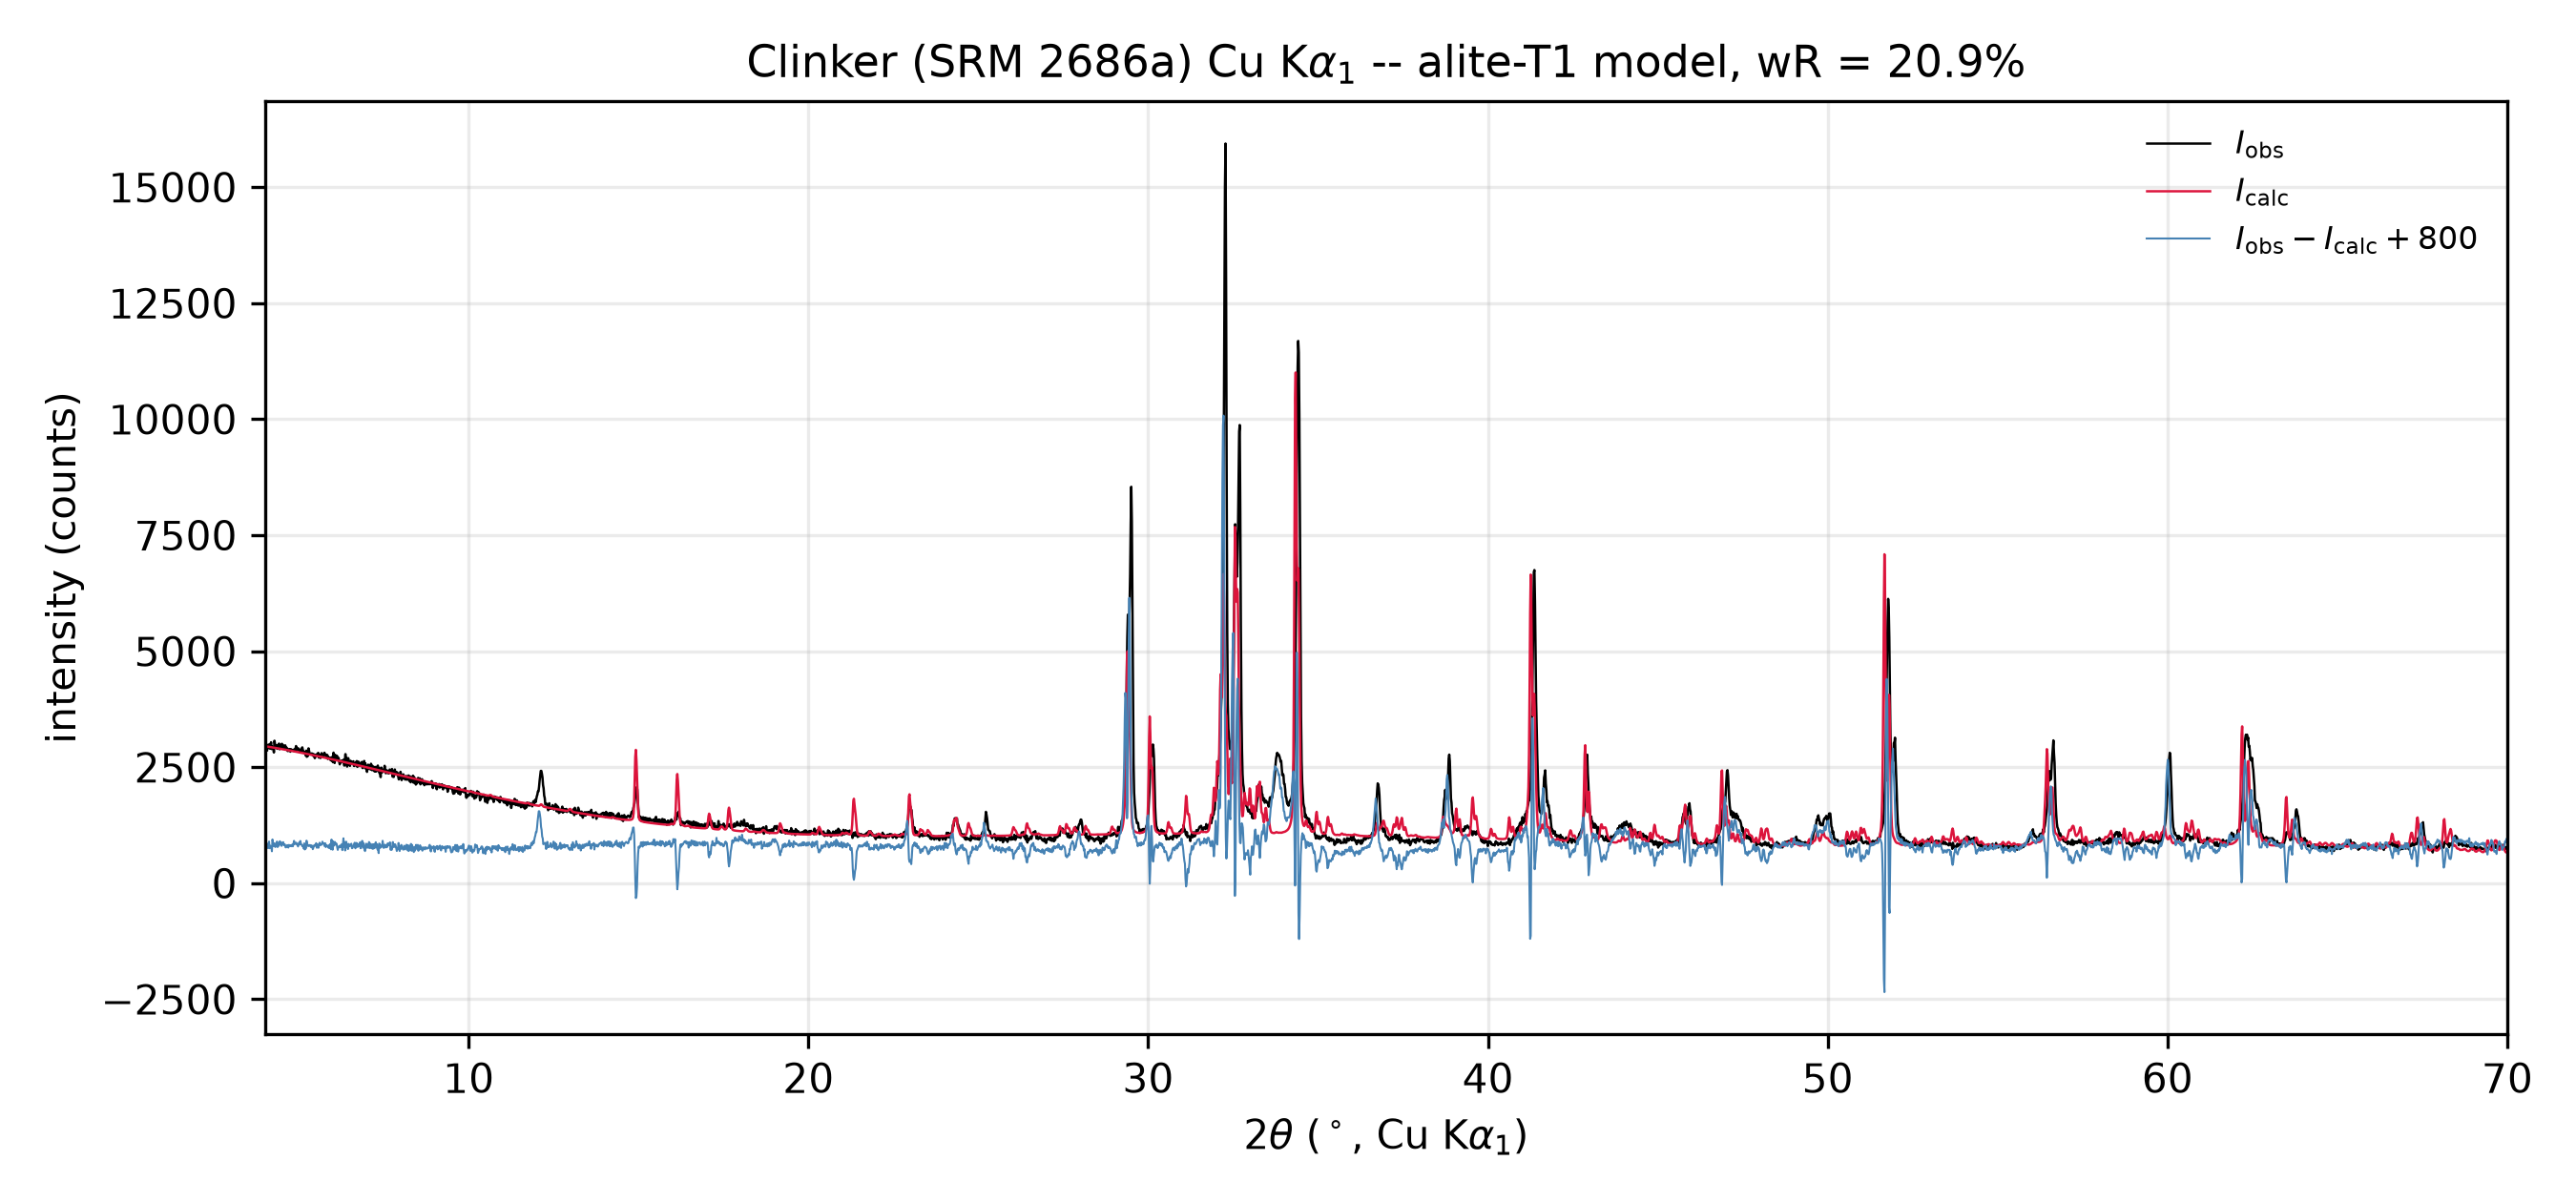
\includegraphics[width=0.96\textwidth]{figures/fig1_clinker_t1_fit.png}
\caption{Clinker Cu pattern with the alite-T1 refinement: observed
(black), calculated (red) and difference (blue, offset
$+800$ counts).}
\label{fig:fit}
\end{figure}

\begin{figure}[ht]
\centering
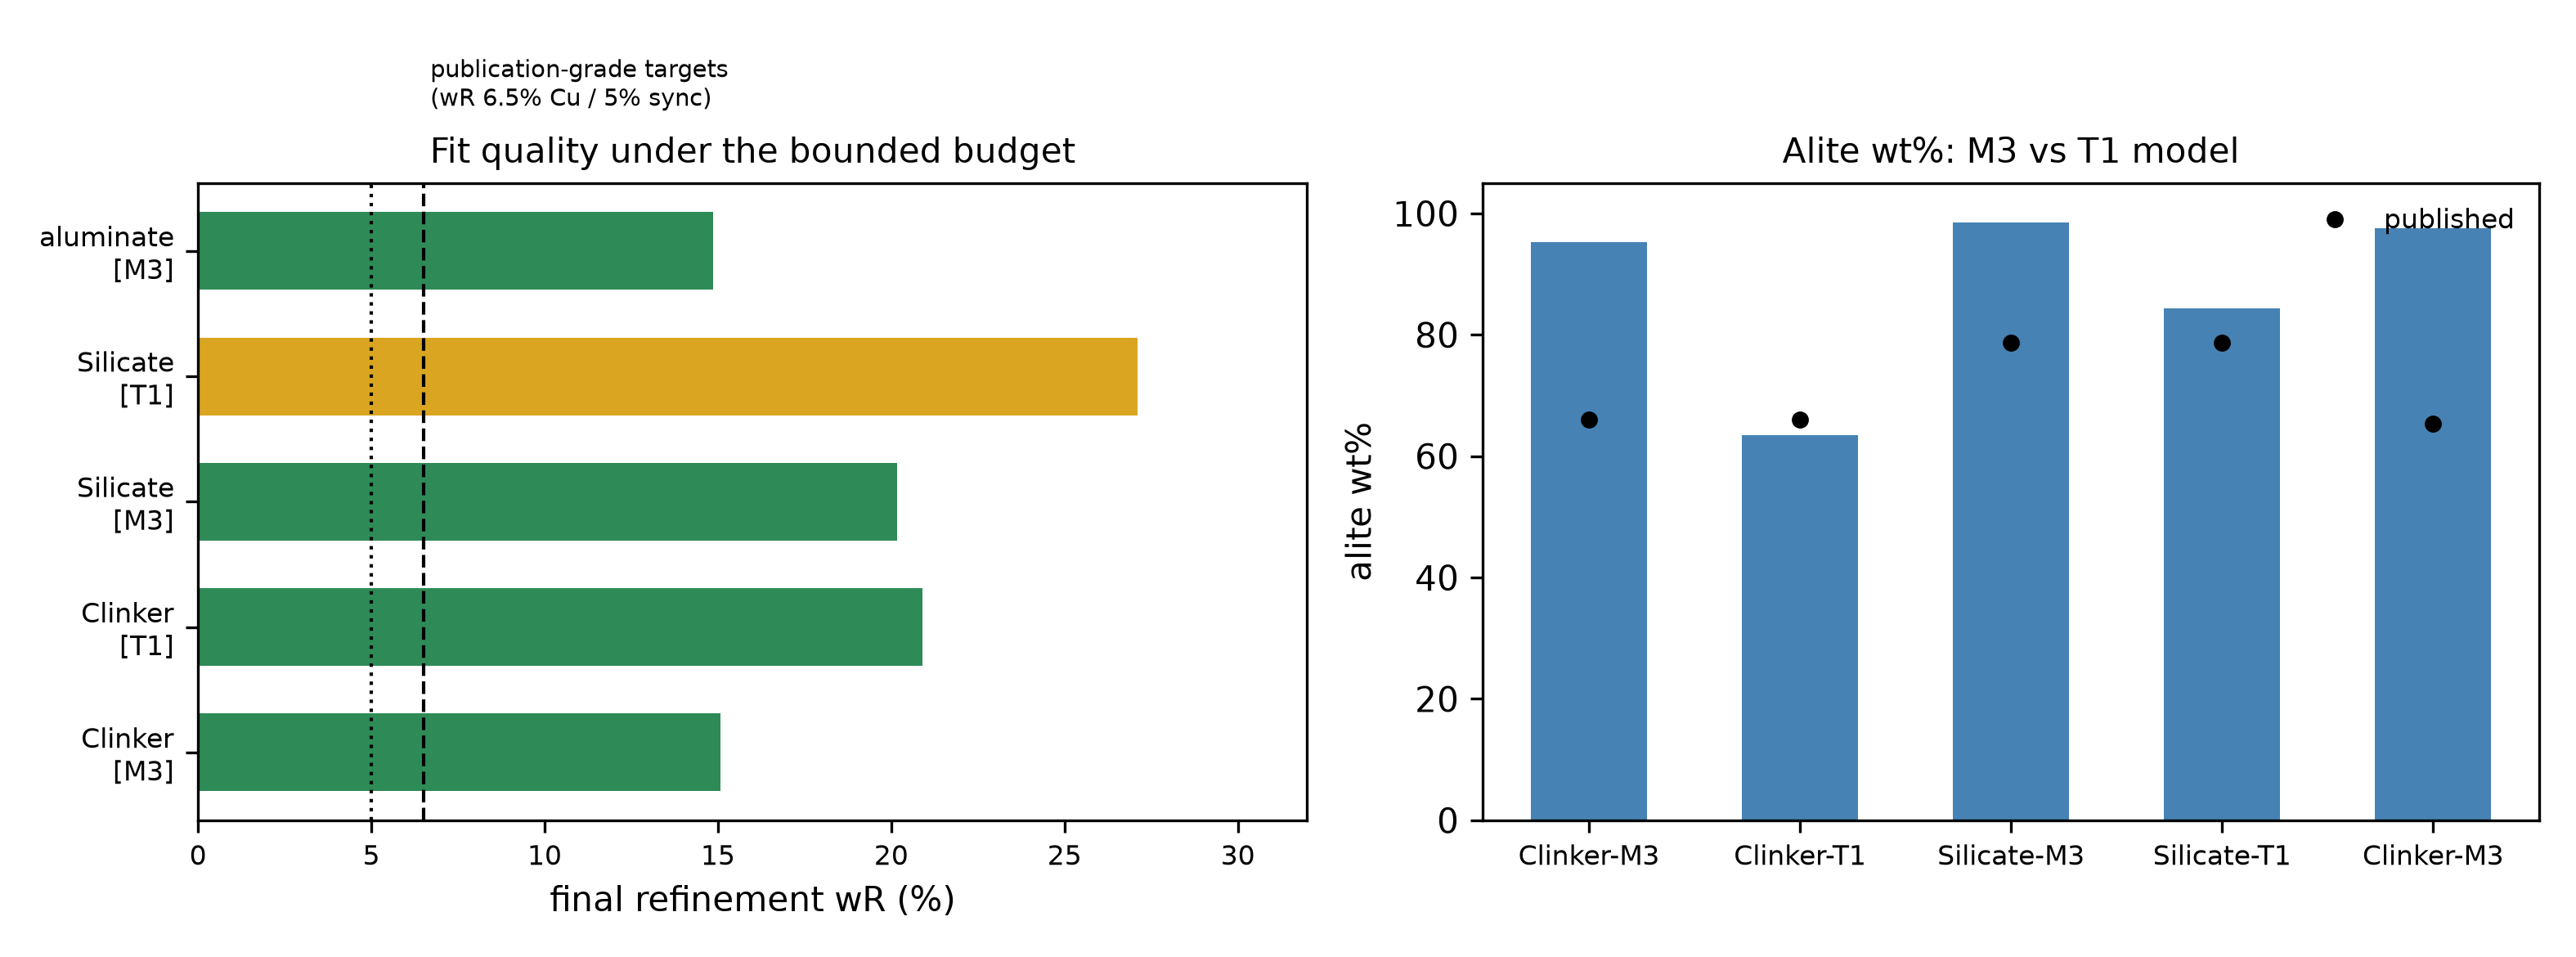
\includegraphics[width=0.96\textwidth]{figures/fig2_results_summary.png}
\caption{Left: final wR per sample/model, with the publication-grade
targets (6.5\% Cu, 5\% sync) marked; right: alite wt\% recovered by the
M3 and T1 models vs.\ the published values.}
\label{fig:summary}
\end{figure}

\section{Discussion and closing}\label{sec:disc}
Two findings matter for the broader RQPA practice. First, the bounded
budget is \emph{deterministic and convergent}: every result in
Table~\ref{tab:results} rebuilds identically via \texttt{make report}
(content hash md5 recorded), which is the property an automated or
agent-driven pipeline needs. Second, the residual per-phase deviations
are physical, not procedural: on synthetic patterns generated from the
same structures at known fractions the same ladder recovers the input
wt\% within the noise floor (Paper P-2), so the real-pattern bias is
attributed to microabsorption --- the target of the repository's planned
Brindley-correction unit 17 --- and is reported honestly rather than
fitted away.

\emph{Closing.} The protocol is the deterministic core of
\texttt{rietveld-agent}; its scientific validity is established
independently in Paper P-2, and its operation from agent runtimes is
described in Paper P-3. This series follows the fifteen-step structure of
\cite{drake2025fifteen}: thesis-first abstract (step 1), story
(step 2), methods and rationale (steps 3--5), CARS introduction
(step 6), findings and problem--response pairs (steps 7--10), and
paragraph/figure planning throughout (steps 11--15).

\section*{License}
Apache-2.0; see \texttt{LICENSE} in the repository root.

\bibliographystyle{plainnat}
\bibliography{references}

\end{document}